\title{Estándares de Usabilidad UI}

\author{\IEEEauthorblockN{Abraham Jhared Flores Azcona}
\IEEEauthorblockA{\textit{Depto. De Sistemas y Computación} \\
\textit{Instituto Tecnológico de Tijuana}\\
Tijuana, Baja California, México \\
abraham.flores193@tectijuana.edu.mx}
}

\maketitle

\begin{abstract}

\end{abstract}

\section{Introducción}

\section{UI}
Las definiciones de UI dependen bastante del nivel de formalidad de la literatura
pertinente. Para las fuentes populares de diseño web y otros tutoriales tales como GeeksForGeeks, tutorialspoint y javatpoint \cite{tutorialspoint-2021,geeksforgeeks-2022,unknown-author-no-dateA} %citarlos
la interfaz de usuario es el la parte visual de una aplicación o sistema operativo a travez de la cual
el usuario interactura con la computadora o la aplicación. En lo que respecta la literatura
académica, \cite{sharma-2021} % TODO citarlos
mencionan que la interfaz de usuario es una interacción entre
el dispositivo y el usuario por medio de técnicas o los comandos para operar el dispositivo,
introducir datos, y usar los contenidos provistos; similarmente, otras publicaciones
coinciden con la definición y agregan que el estudio de UI se realiza de manera complementaria al UX \cite{joo-2017,guntupalli-no-date}% TODO citar a Joo y a Guntupalli
(el cual ya se mencionó en la asignación anterior).
\\

En ambas esferas de conocimiento, el consenso general se puede resumir en el poder birndar al usuario una
manera de ``moverle a la compu'' sin mucho problema.

\section{Usabilidad}
La usabilidad es una medida que de acuerdo a la Fundación de Diseño de Interacción \cite{unknown-author-no-dateC}, % TODO citar a la fundación
permite a un usuario específico utilizar un producto/diseño en un contexto dado para lograr
un objetivo especifico de manera efectiva, eficiente y satisfactoriamente. \cite{unknown-author-no-dateB} menciona % TODO citarlo
que dicha usabilidad es un atributop cualitativo, por lo que tendremos inherentemente una
evaluación sesgada, sin embargo lista cinco elementos que concretan la definición:
(1) Facilidad de aprendizaje, (2) Eficiencia, (3) Facilidad de memorización, (4) Errores 
y (5) Satisfacción.
\\

Otras definiciones, como la de \cite{guntupalli-no-date} % TODO citarlo
incluyen que la usabilidad (en el contexto de las interfaces de usuario),
es compuesta de tres disciplinas del diseño: De interacción, de información y de 
interfaz, como se muestra en la Fig. \ref{fig:fig1}. El diseño de información destaca
bastante debido a no ser frecuentemente mencionado como parte del diseño de la usabilidad
en distintos articulos. Se define como la forma en que se muestran los datos que permiten 
al usuario discernir si son relevantes para la tarea a realizar; si se desea evaluar la usabilidad,
es de igual importancia conocer las métricas que nos permitan medir la interacción, la información
y la interfaz para sus posibles mejoras, sin embargo, las metricas que meciona son de caracter 
cualitativo y son las mencionadas en la Tabla \ref{tab1}.
\begin{table}[t]
    \caption{Métricas cualitativas para crear un diseño de interfaz eficiente.}
    \begin{center}
        \begin{tabular}{c c}
        \hline
        \textbf{Núm. regla} & \textbf{Descripción}\\
        \hline
        1 & Consistencia del programa\\
        2 & Atajos\\
        3 & Retroalimentación\\
        4 & Cuadros de diálogo\\
        5 & Recuperabilidad\\
        6 & Función de \emph{undo}\\
        7 & Control del programa\\
        8 & Facilidad de memorización\\
        \hline
        \end{tabular}
    \end{center}
    \label{tab1}
\end{table}
\begin{figure}[t]
    \centering
    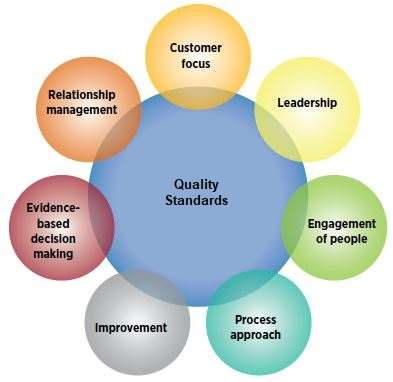
\includegraphics[scale=0.45]{../images/fig1.png}
    \caption{Disciplinas que conforman la usabilidad.}
    \label{fig:fig1}
\end{figure}
\\

Otras consideraciones importantes que \cite{joo-2017}  % TODO citarla
menciona son aquellas de las areas para el diseño mas apropiado de una UI/UX que consisten en:
(1) El conocimiento básico de UI/UX, (2) Establecer los puntos a investigar para el diseño,
(3) Establecer el concepto unificador de diseño como lo es las palabras clave del producto y
(4) El diseño de la producción, que considera aspectos técnicos tales como la resolución y la tipografía.

\subsection{Metricas de Usabilidad}
Debido que la usabilidad se define junto a mediciones, es igualmente necesario conocer que métricas son
importantes. Para la explicación y el análisis de las métricas, utilizaremos aquellas mencionadas en \cite{kokol-1995,purchase-2011,hentati-2015} % TODO citar a Hentati et al., Kokol et al. y Hilbert y Redmiles
debido al nivel de profundidad mostrado en sus explicaciones asi como las evidencias estadísticas
que refutan la vericidad de las mismas.
\\

\section{Ejemplo: reddit}
reddit es una plataforma que le permite a los usuarios crear foros (llamados \emph{subreddits}) y
publicar, comentar, compartir y votar contenidos provenientes dentro o fuera de la plataforma.
\begin{figure}[t]
    \centering
    
\includegraphics[scale=0.33]{../images/fig2.png}
    \caption{Despliegue de inicio de usuario de reddit.}
    \label{fig:fig2}    
\end{figure}
\\

Es importante destacar que la interfaz a analizar es aquella del \emph{new} reddit (Fig. \ref{fig:fig2}), que es
más familiar con otras páginas web contemporaneas, mientras que su contraparte de \emph{old}
reddit es la versión original del sitio, que se caracteríza por ser muy parecida a las paginas
web de los 90s. Debido a las métricas tan variadas que fueron expuestas anteriormente, se analizará
la interfaz por medio de tres métricas diferentes.
\\


\section{Conclusión}

\bibliographystyle{IEEEtran}
\bibliography{bibliography}